\documentclass{math_library}

\begin{document}
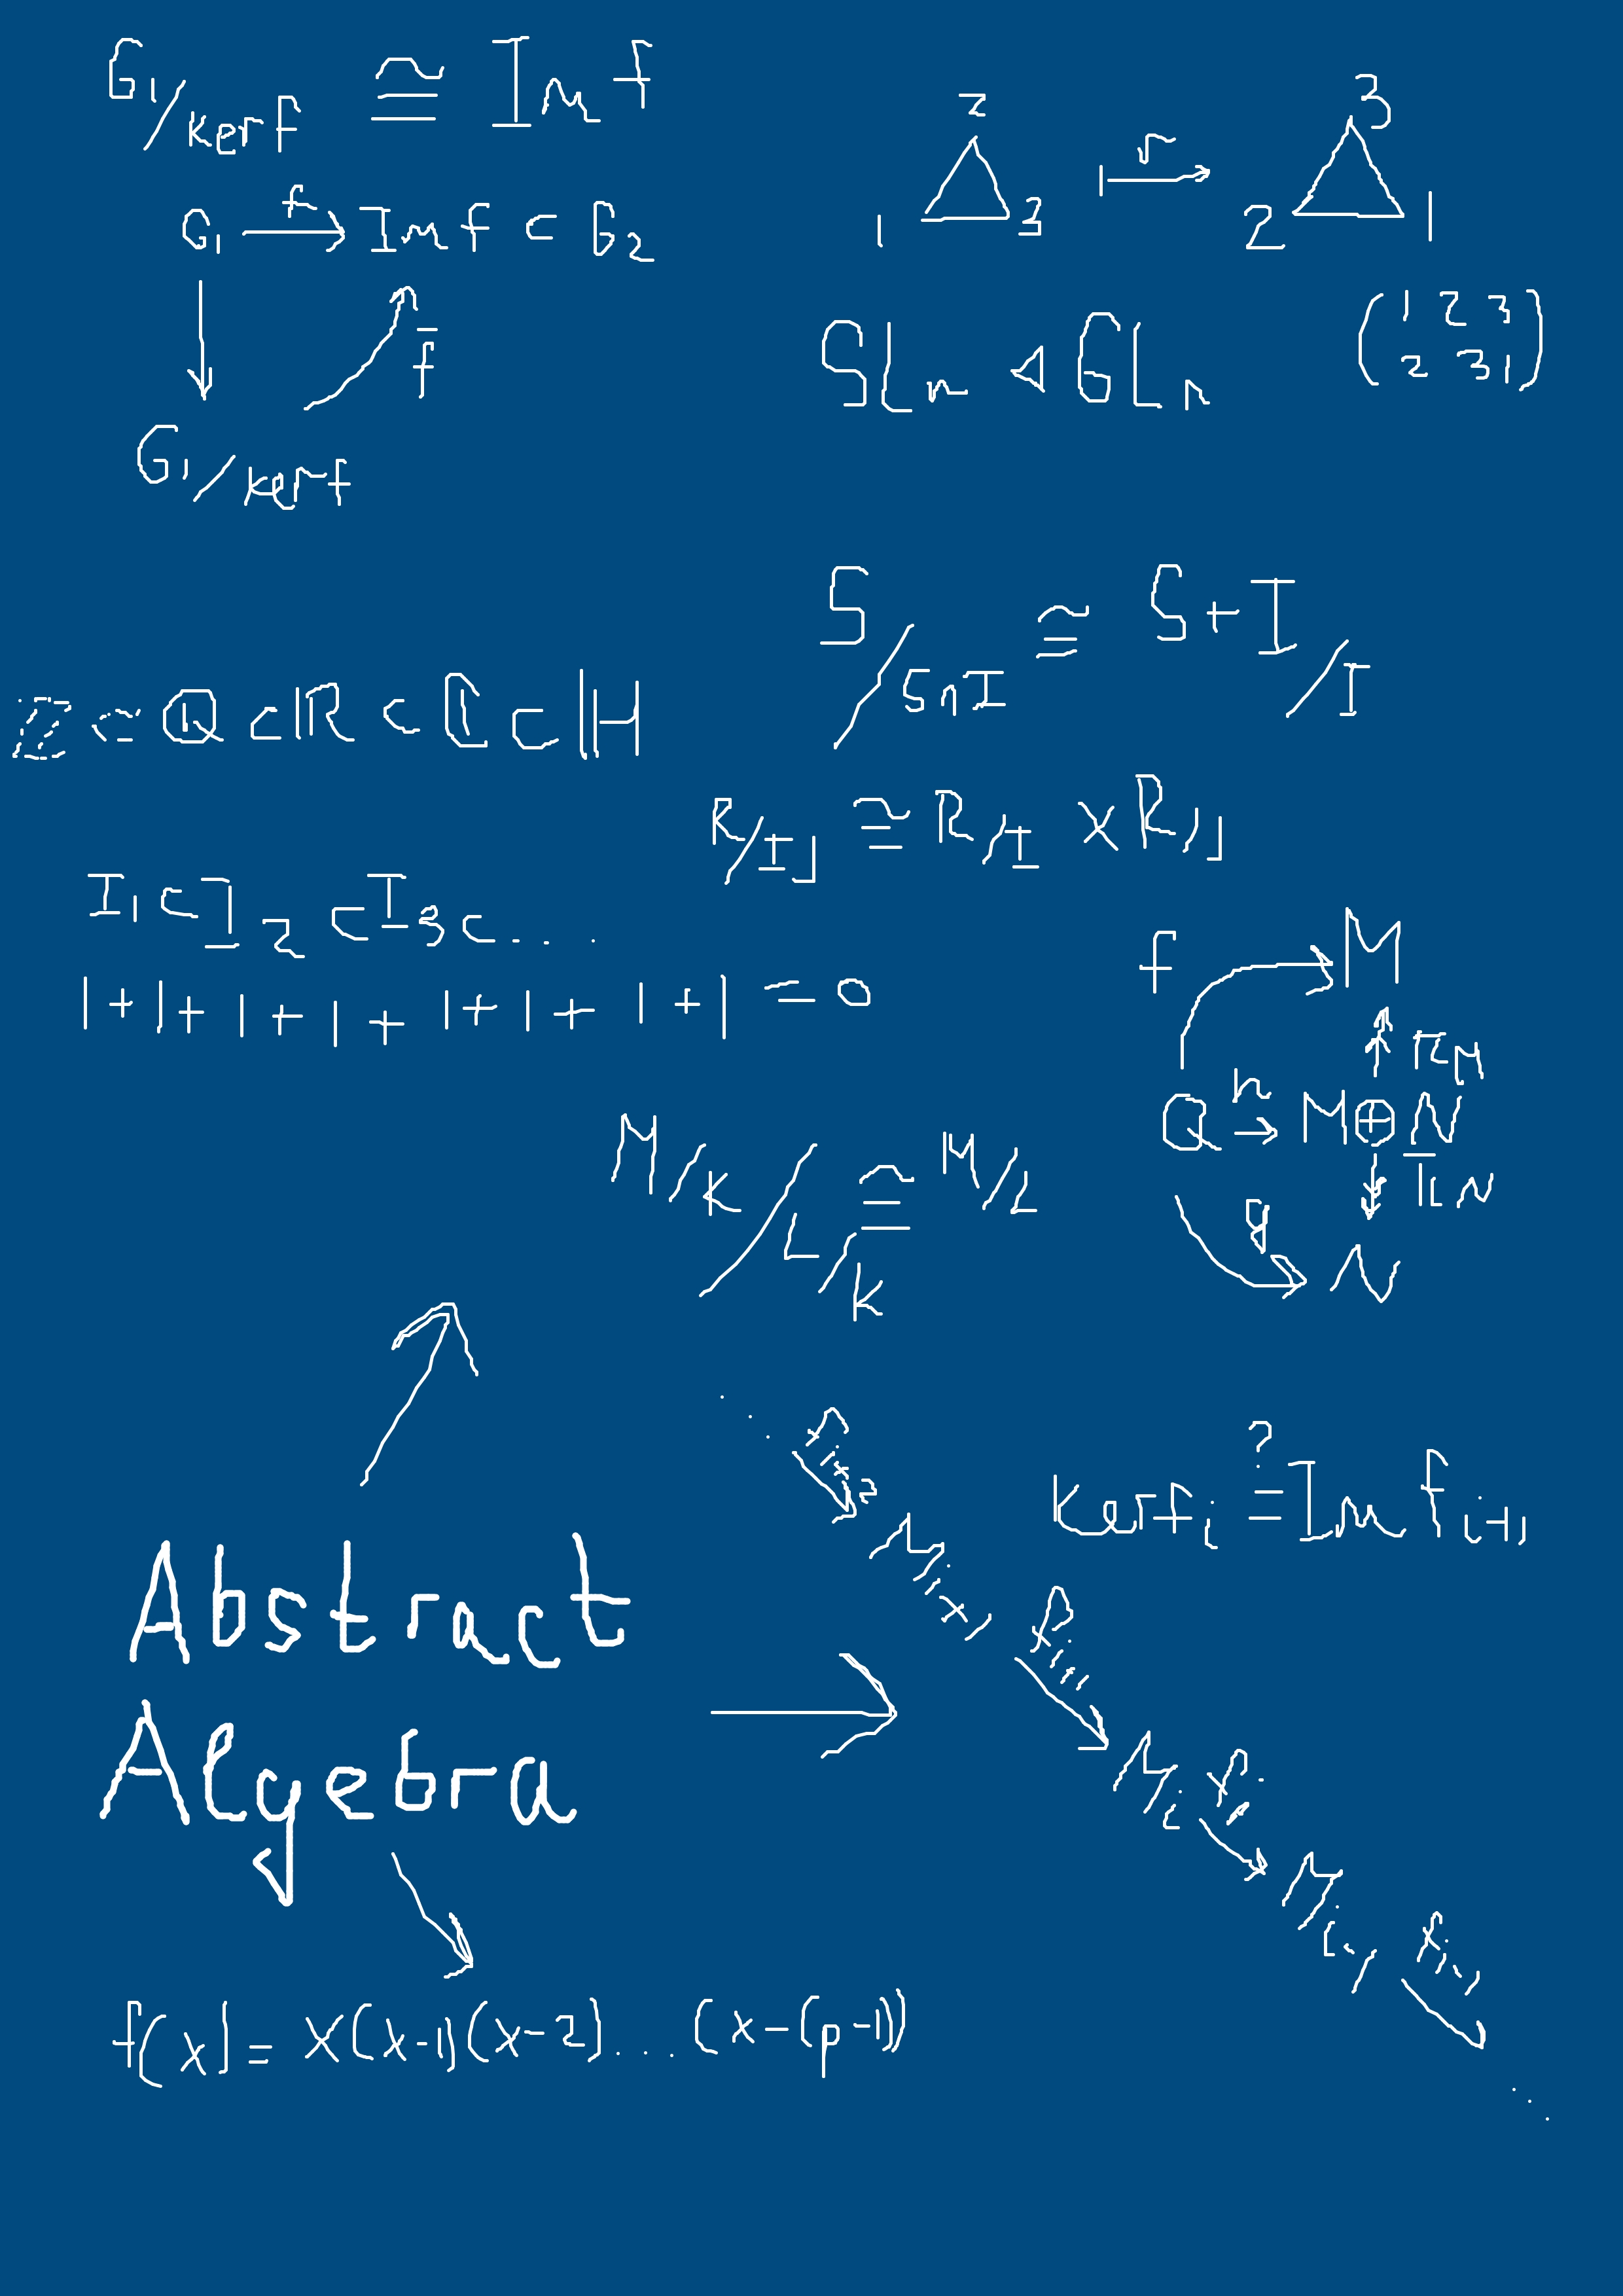
\includepdf[scale=1]{preview.jpg}

\section*{Повторення матеріалу}
\newpage

\section{Теорія груп}

\subsection{Означення груп}
\begin{enumerate}[wide=0pt,label=\thesubsection.\arabic*]
\item Перевірити, чи буде задана структура задавати групу:
\begin{itemize}[nosep,wide=0pt]
\item $\left< \mathbb{N}, + \right>$;
\item $\left< \mathbb{R}, \cdot \right>$;
\item $\left< \mathbb{Q}(\sqrt{2}), \cdot \right>$, де множина $\mathbb{Q}(\sqrt{2}) = \{ a+b \sqrt{2} \mid a, b \in \mathbb{Q}, \text{ ненульові одночасно} \}$.
\end{itemize}

\item Нехай $\left<G,*\right>$ --- група. Довести, що $(a^{-1})^{-1} = a$ для будь-якого $a$.

\item Нехай $\left<G,*\right>$ --- група. Довести, що справедлива рівність $(a*b)^{-1} = b^{-1}*a^{-1}$. Внаслідок чого переконатися, що $(a_1*a_2*\dots*a_n)^{-1} = a_n^{-1}* \dots *a_2^{-1}*a_1^{-1}$.

\item Доведіть, якщо $g^2 = e$ виконується для всіх $g \in G$, то $\left<G,*\right>$ --- абелева.

\item Розгляньте кожний випадок, коли множина $G$ містить: $1$ елемент, $2$ елементи, $3$ елементи та $4$ елементи. Довести, що для перших трьох існує лише одне можливе множення $* \colon G \times G \to G$, для якого $\left<G,*\right>$ буде групою (\textit{а що з останнім випадком?}). Чи будуть всі ці групи абелевими? 
\end{enumerate}

\subsection{Деякі інші корисні групи}
\subsubsection{Групи лишків}
\begin{enumerate}[wide=0pt,label=\thesubsection.\arabic*]
\item У групі $\left<\mathbb{Z}_8,+\right>$ обчислити наступне:
 \begin{itemize}[nosep,wide=0pt]
\item $\overline{2} + \overline{-10} + \overline{2025}$;
\item $\overline{1} \cdot \overline{2} \cdot \overline{3} \cdots \overline{\the\year}$;
\end{itemize}

\item Розв'язати рівняння $\overline{2} \cdot \overline{x} = \overline{4}$ в групі $\left<\mathbb{Z}_8,+\right>$.

\item Знайти елементи для групи $\left< U_{18}, \cdot \right>$.

\item Довести, що квадрат будь-якого непарного числа в $\mathbb{Z}_8$ дорівнює $\overline{1}$.

\item Знайти останню цифру числа $\the\year^{{\the\year+1}}$ (\textit{вказівка: знайти останню цифру означає знайти остачу при діленні на $10$, а для цього треба це число розглянути в групі $\mathbb{Z}_{10}$}).

\item Довести теорему Вілсона: $p$ --- просте число $\iff (p-1)! \equiv -1 \pmod p$ (\textit{вказівка: \rightproof покажи, що обернені самому собі є елементи $\overline{1},\overline{p-1}$; \leftproof припусти, що $p$ --- не просте}).
\end{enumerate}

\subsubsection{Дієдричні групи}
\begin{enumerate}[wide=0pt,label=\thesubsection.\arabic*, start=6]
\item У дієдричній групі $\left< D_4, \circ\right>$ спростити вираз:
\begin{itemize}[nosep,wide=0pt]
\item $r^{\the\year} s^3$;
\item $s^{-1} r^{-4} s^6 r^{13}$.
\end{itemize}

\item Можна, насправді кажучи, визначити дієдричну групу $D_2$ --- група симетрії так званого $2$-кутника (\textit{це просто відрізок}). Описати всі можливі симетрії над відрізком, внаслідок чого описати $D_2$. Довести, що $D_2$ --- абелева група.
\end{enumerate}

\subsubsection{Група кватерніонів}
Довести, що $\left< Q_8, \cdot\right>$ із множенням, $i^2 = j^2 = k^2 = ijk = -1$ задає групу.

\subsubsection{Групи симетрій}
(TODO: вигадати задачі)

\subsection{Підгрупи}
\begin{enumerate}[wide=0pt,label=\thesubsection.\arabic*]
\item Довести, що:
\begin{itemize}[nosep]
\item $\mathbb{Z}$ є підгрупою групи $\left<\mathbb{R},+\right>$;
\item $\mathrm{SL}_n(\mathbb{R})$ є підгрупою групи $\mathrm{GL}_n(\mathbb{R})$;
\item $O(n)$ є підгрупою групи $\mathrm{GL}_n(\mathbb{R})$, де $O(n) = \{A \in \Mat_{n \times n}(\mathbb{R}) \mid A^T A = I \}$.
\item $S^1$ є підгрупою групи $\mathbb{C}$, де $S^1 = \{z \in \mathbb{C} \mid |z| = 1\}$;
\item $\text{LFT}(\bar{\mathbb{C}})$ є підгрупою $S_{\bar{\mathbb{C}}}$. Нагадаю, що $S_{\bar{\mathbb{C}}}$ --- група всіх бієкцій $\bar{\mathbb{C}} \to \bar{\mathbb{C}}$, а також $\text{LFT}(\bar{\mathbb{C}})$ --- множина всіх дробово-лінійних відображень (\textit{див. комплексний аналіз}).
\end{itemize}

\item Нехай $\left<G,*\right>$ --- абелева група та $n \in \mathbb{N}$. Довести, що множина $H = \{ g^n \mid g \in G\}$ утворює підгрупу $G$ (\textit{чи можна сказати в зворотному напрямку?}).

\item Задано групу $\left< G,*\right>$ та деяку сім'ю підгруп $\{H_\alpha\}$ групи $G$ (\textit{можливо, нескінченна сім'я}). Покажіть, що $\displaystyle\bigcup_{\alpha} H_\alpha$ --- не обов'язково підгрупа $G$. Для цієї задачі є продовження:
\begin{itemize}[nosep,wide=0pt]
\item Нехай $H,H'$ --- підгрупи $G$. Довести, що $H \cup H'$ --- підгрупа $G \iff H \subset H'$ або $H \supset H'$;
\item Якщо $H_0 \subset H_1 \subset H_2 \subset \dots$ --- ланцюг підгруп $G$, довести, що $\displaystyle\bigcup_{\alpha} H_\alpha$ буде підгрупою $G$.
\end{itemize}
\end{enumerate}

\subsection{Підгрупи, породжені множиною}
\begin{enumerate}[wide=0pt,label=\thesubsection.\arabic*]
\item Довести, що група $\left< S_n, \circ \right>$ породжена транспозиціями.

\item Довеси, що група $\mathrm{SL}_2(\mathbb{Z})$ породжена матрицями $\begin{pmatrix}
0 & -1 \\
1 & 0
\end{pmatrix},\ \begin{pmatrix}
1 & 1 \\
0 & 1
\end{pmatrix}$.
\end{enumerate}

\subsection{Циклічні підгрупи}
\begin{enumerate}[wide=0pt,label=\thesubsection.\arabic*]
\item Нехай $G$ --- скінченна група, яка містить лише єдиний елемент $x \in G$, для якого $\ord (x) = 2$. Довести, що $\displaystyle\prod_{g \in G} g = x$.

\item Нехай $\ord(g)$ --- непарне. Що можна сказати за $\ord(g^2)$? \phantom{(теж непарне)}

\item Для будь-яких $g,h \in G$ довести, що $\ord(g*h) = \ord(h*g)$ (\textit{вказівка: доведіть, що $\ord(a*g*a^{-1}) = \ord(g)$ для всіх $a,g \in G$}).

\item Розглянемо матриці $A = \begin{pmatrix}
0 & -1 \\
1 & 0
\end{pmatrix},\ B = \begin{pmatrix}
0 & 1 \\
-1 & -1
\end{pmatrix}$. Довести, що $\ord(A) = 4,\ \ord(B) = 3$, проте $\ord(AB) = \infty$.

\item Для кожного $n \in \mathbb{N}$ побудувати групу, що містить два елементи $g,h$ так, що $\ord(g) = 2,\ \ord(h) = 2$, а також $\ord(gh) = n$ (\textit{вказівка: глянути на $D_n$}).

\item Довести, що $\left< \mathbb{Q},+\right>$ --- нециклічна група.
\end{enumerate}

\subsection{Гомоморфізм груп}
\begin{enumerate}[wide=0pt,label=\thesubsection.\arabic*]
\item Довести, що група $G$ порядка $n$ ізоморфна $\mathbb{Z}_n \iff G$ містить елемент порядка $n$. 

\item Довести, що $\mathbb{C} \setminus \{0\} \not\cong \mathbb{R} \setminus \{0\}$.

\item Нехай $G$ --- група. Довести, що $\varphi \colon G \to G$, що задана як $\varphi(g) =g^{-1}$ --- ізоморфізм $\iff G$ --- абелева.

\item Знайти всі гомоморфізми $f \colon \mathbb{Z}_9 \to \mathbb{Z}_{15}$.
\end{enumerate}

\subsection{Ядра, образи гомоморфізмів}
\begin{enumerate}[wide=0pt,label=\thesubsection.\arabic*]
\item Знайти ядро та образ гомоморфізма $\det \colon \textrm{GL}_n \to \mathbb{R} \setminus \{0\}$.
\end{enumerate}

\subsection{Суміжні класи}
\begin{enumerate}[wide=0pt,label=\thesubsection.\arabic*]
\item Нехай $G$ --- група та $H,K \leq G$, що мають скінченний індекс. Тоді $H \cap K$ також має скінченний індекс.
\end{enumerate}

\subsection{Нормальні підгрупи}
\begin{enumerate}[wide=0pt,label=\thesubsection.\arabic*]
\item Серед підгруп $S_3$ вказати, які є нормальними, а які --- ні.

\item Нехай $\left<G,*\right>$ --- група та $H \leq G$ так, що $[G:H] = 2$. Довести, що $H \triangleleft G$.

\item Для груп $\left< G, * \right>$ нехай відомо, що $K \triangleleft H$ та $H \triangleleft G$. Чи випливає з цього, що $K \triangleleft G$? (\textit{вказівка: подивитись на групу $D_4$ та на якісь дві підгрупи}).

\item Нехай $G$ --- група та $H \triangleleft G$. Довести, що $G/_H$ --- абелева $\iff [g,h] \in H$ (\textit{елемент $[g,h] = g*h*g^{-1}*h^{-1}$ називається комутатором}).
\end{enumerate}

\subsection{Факторгрупи}
\begin{enumerate}[wide=0pt,label=\thesubsection.\arabic*]
\item Нехай $G_1,G_2$ --- дві групи, які містять підгрупи, що ізоморфні $H$. Припустимо, що $G_1/_H \cong G_2/_H$. Чи правда, що $G_1 \cong G_2$? (\textit{вказівка: Кляйн viergruppe та інша група порядка $4$}).
\end{enumerate}

\subsection{Прямі добутки}
\begin{enumerate}[wide=0pt,label=\thesubsection.\arabic*]
\item Довести, що $G_1 \times G_2$ утворює групу з операцією, визначеною на лекції.

\item Нехай $G_1,G_2$ --- групи. Припустимо, що $K \leq G_1 \times G_2$. Чи обов'язково $K$ має вигляд прямого добутку $H_1 \times H_2$, де $H_1 \leq G_1,\ H_2 \leq G_2$? (\textit{вказівка: розглянути $G_1,G_2$ як групи з двома елементами}).

\item Нехай $G$ --- скінченна група, причому кожен елемент є сам собі оборотним. Довести, що $G \cong \mathbb{Z}_2 \times \dots \times \mathbb{Z}_2$.
\end{enumerate}

\subsection{Теореми про ізоморфізми}
\begin{enumerate}[wide=0pt,label=\thesubsection.\arabic*]
\item Нехай $G$ --- скінченна група та $n > 1$, причому $(xn)^n = x^n y^n$ для всіх $x,y \in G$. Позначимо
\[
G[n] = \{g \in G: g^n = 1\}, \qquad G^n = \{ g^n \mid g \in G\}.
\]
Довести, що $G[n], G^n \triangleleft G$. Крім того, показати, що $|G^n| = [G:G[n]]$.
\end{enumerate}
\newpage

\section{Теорія групової дії}
\subsection{•}
\subsection{•}
\subsection{•}
\subsection{•}
\subsection{•}
\subsection{•}
\subsection{•}
\subsection{Нормалізатори}
\begin{enumerate}[wide=0pt,label=\thesubsection.\arabic*]
\item Нехай $H \leq K \leq G$. Довести, що $N_K(H) = N_G(H) \cap K$.

\item Довести, що $N_G(aHa^{-1}) = aN_G(H)a^{-1}$. Іншими словами це сформулювати можна так: якщо $H_1,H_2$ --- спряжені підгрупи, то $N_G(H_1),N_G(H_2)$ --- спряжені також.
\end{enumerate}

\subsection{$p$-групи та деякі результати}
\begin{enumerate}[wide=0pt,label=\thesubsection.\arabic*]
\item Спростувати твердження: якщо $G$ --- група, де $|G| = p^k$, то $G$ --- абелева при $k \geq 3$ (\textit{при $k \in \{0,1,2\}$  всім же відомо, що це виконується?}). Для цього:
\begin{itemize}[wide=0pt]
\item при $p = 2$ розгляньте дієдричну групу (\textit{але який правильний $n$-кутник треба взяти?});
\item при непарних $p$ треба розглянути групу Гайзенберга
\[
H(p) = \left\{ \begin{pmatrix}
1 & a & b \\
0 & 1 & c \\
0 & 0 & 1
\end{pmatrix} \mid a,b,c \in \mathbb{Z}_p \right\}.
\]
Що можете сказати за групу $G = H(p) \times \mathbb{Z}_{p^{k-3}}$?

\item Нехай $|G| = pq$, де $p,q$ --- прості числа.
\end{itemize}
\end{enumerate}
\subsection{Теорема Коші та теореми Сілова}
\begin{enumerate}[wide=0pt,label=\thesubsection.\arabic*]
\item Нехай $G$ --- скінченна група, причому для кожного $p \mid |G|$ існує лише одна $p$-Сіловська підгрупа. Довести, що $G$ є (внутрішнім) прямим добутком його Сіловських підгруп.
\end{enumerate}
\newpage

\section{Ряди підгруп}
\subsection{Комутанти}
\begin{enumerate}[wide=0pt,label=\thesubsection.\arabic*]
\item Довести властивості, які були в якості вправи:
\begin{itemize}
\item $x*y = [x,y]*(y*x)$;
\item $x,y$ комутують між собою $\iff [x,y] = e$;
\item $[x,y]^{-1} = [y,x]$;
\item $\forall g \in G: [x^g,y^g] = [x,y]^g$;
\item Нехай $\left< H,\star\right>$ --- ще одна група та $\varphi \colon G \to H$ --- гомоморфізм груп. Тоді $\varphi([x,y]) = [\varphi(x),\varphi(y)]$.
\end{itemize}

\item Довести, що матриця $\begin{pmatrix}
-1 & 0 \\
0 & -1
\end{pmatrix}$ не записується як комутатор двох матриць в групі $\mathrm{SL}_2(\mathbb{R})$.
\bigskip \\
%deep explanation
!Припустимо, що виконується така рівність:
\[
\begin{pmatrix}
-1 & 0 \\
0 & 1
\end{pmatrix} = ABA^{-1}B^{-1} \implies \begin{pmatrix}
-1 & 0 \\
0 & 1
\end{pmatrix} BA = AB.
\]
Для зручності позначимо матриці
\[
A = \begin{pmatrix}
a & b \\
c & d
\end{pmatrix}, \qquad B = \begin{pmatrix}
w & x \\
y & z
\end{pmatrix}.
\]
Тоді отримаємо систему:
\[
\begin{cases} 
2aw + by + cx & = 0; \\
ax + bw + bz + dx & = 0; \\
ay + cw + cz + dy & = 0; \\
by + cx + 2dz & = 0; \\
ad - bc & = 1; \\
wz - yx & = 1.
\end{cases}
\]
Останні два рівняння --- це з умови $A,B \in \mathrm{SL}_2(\mathbb{R})$.\\
Якщо $a = 0$, то тоді розв'язок уже неможливий; при $d = 0$ уже маємо $b,c \neq 0$ в силу передостаннього рівняння --- отримаємо систему 
\[
\begin{cases} 
cx + by & = 0; \\
 w & = -z; \\
 bc & = -1; \\
 wz - xy & = 1.
 \end{cases}
\] Але тоді звідси $y = c^2 x$, тож отримаємо $-z^2 - c^2y^2 = 1$ --- така рівність неможлива. При $d \neq 0$ через Гауса отримаємо $z = w = 0$, а після цього $x = 0$, що уже неможливо для $B \in \mathrm{SL}_2(\mathbb{R})$.\\
Аналогічно $d = 0$ призведе до неможливості розв'язку. При $b = 0$ або $c = 0$, там буде трошки по-іншому, але теж розв'язків нема.\\
Отже, надалі $a,b,c,d \neq 0$.\\
Пройдемось по методу Гауса (\textit{розв'язуючи систему відносно $w,x,y,z$}). Якщо $-2a^2 -ad - 1 = 0$, то можемо виразити $d$. Знаючи $ad - bc = 1$, можемо добити метод Гауса та отримати, що четвертий рядок та четвертий стовпчик матриці має елемент $\dfrac{8a^4+2a^3+10a^2+a+1}{a}$, який додатний. Тоді ранг матриці максимальний, що неможливо (бо тоді $w,x,y,z = 0$).\\
Якщо $-2a^2 - ad - 1 \neq 0$, то продовжимо метод Гауса. Там можливо буде скоротити на $a + d$, бо він нулем не може бути. Отримаємо методом Гауса $a^3d - a^3cd + ad + 1$, а решта діагональні елементи ненулеві. Якщо $a^3d - a^3cd + ad + 1 \neq 0$, то ранг максимальний (\textit{неможливо}). Тому окремо $a^3d - a^3cd + ad + 1 = 0$. На моменті Гауса в нас буде
\[
\begin{pmatrix}
2a & c & b & 0 \\
0 & -2a^2-ad-1 & b^2 & -2ab \\
0 & 0 & (a^2+1) & ac \\
0 & 0 & 0 & a^3d - a^2cd +ad +1
\end{pmatrix}.
\]
Далі лінь рахувати, але там теж не вийде розв'язків.
\iffalse
$\begin{pmatrix}
2a & c & b & 0 \\
b & a+d & 0 & b \\
c & 0 & a+d & c \\
0 & c & b & 2d
\end{pmatrix} \sim \begin{pmatrix}
2a & c & b & 0 \\
0 & cb - 2a(a+d) & b^2 & -2ab \\
0 & c^2 & bc-2a(a+d) & -2ac \\ 
0 & c & b & 2d
\end{pmatrix} \sim \\
\sim \begin{pmatrix}
2a & c & b & 0 \\
0 & -2a^2-ad-1 & b^2 & -2ab \\
0 & c^2 & -2a^2-ad-1 & -2ac \\ 
0 & c & b & 2d
\end{pmatrix} \sim \\
\sim \begin{pmatrix}
2a & c & b & 0 \\
0 & -2a^2-ad-1 & b^2 & -2ab \\
0 & 0 & (a+d)(a^2+1) & ac(a+d) \\
0 & 0 & ad(a+d) & (a+d)(ad+1)
\end{pmatrix} \sim \\
\sim \begin{pmatrix}
2a & c & b & 0 \\
0 & -2a^2-ad-1 & b^2 & -2ab \\
0 & 0 & (a^2+1) & ac \\
0 & 0 & 0 & a^3d - a^2cd +ad +1
\end{pmatrix}$.\\
\fi

\item Знайти, чому дорівнює $Q_8'$, а також абеліанізацію $(Q_8)_{\text{ab}}$.

\item Знайдемо знайти комутатор для групи 
\[
G = \left\{ \begin{pmatrix}
1 & a & 0 \\
0 & 1 & 0 \\
0 & b & c
\end{pmatrix} \Big| a,b,c \in \mathbb{R}, c \neq 0 \right\}.
\] 

\item Довести, що $A_n' = A_n$ при $n \geq 5$ (\textit{вказівка: треба будь-який $3$-цикл $(ijk)$ розписати як комутатор}). Що не так при $n = 3$ та $n = 4$?
\iffalse
\bigskip \\
$[(ij) \cdot (lm),\ (jk) \cdot (lm)] = (ikj)$.
\fi
\end{enumerate}
\end{document}
